\chapter{Mineração Web}
A mineração web utiliza muitos conceitos da mineração de dados tradicional, por isso para começarmos a falar do assunto principal deste trabalho, que é a Mineração Web, teremos que introduzir alguns termos e conhecimentos mínimos de entendimento necessário para facilitar a compreensão.

\section{Mineração de Dados}

	Segundo \cite{BingLiu}, Mineração de Dados ou Data mining é o processo de analisar um grande conjunto de dados com o objetivo de encontrar padrões, informações relevantes. Devido à grande quantidade de dados que existem hoje em dia, geralmente não é mais possível fazer a análise individual dos dados para então obter-se alguma informação. Para solucionar esse problema, utilizamos a mineração de dados  que é capaz de fazer essa análise em uma grande quantidade de dados. A mineração de dados é uma iteração das seguintes etapas:

\begin{itemize}
\item 	Pré-processamento: nesta etapa é feita uma preparação dos dados recolhidos, ou seja, os dados são analisados e ruídos são retirados, pois geralmente não estão devidamente adequados para mineração logo após o recolhimento;
\item 	Mineração: após o pré-processamento o dado será então minerado pelo algoritmo que produzirá padrões e conhecimentos;
\item  	Pós-processamento: para finalizar é feita a identificação e seleção dos padrões úteis para a pesquisa, já que muitas vezes os padrões encontrados pelo algoritmo não são úteis.
\end{itemize}

Apesar de utilizar muitos fundamentos da mineração de dados tradicional, existem algumas diferenças entre esta e a mineração web, sendo a principal delas é que a primeira aplica a mineração em dados estruturados, organizados em tabelas, como em um banco de dados, e a segunda em dados não-estruturados ou semi-estruturados.


\section{A Mineração Web}
	Segundo \cite{BingLiu}, web mining é o uso das técnicas de data mining para descobrir e extrair automaticamente informações relevantes dos documentos e serviços ligados a internet.

	Este tipo de mineração utiliza as técnicas de data mining, com algumas modificações já que os dados na web não são estruturados, para extrair automaticamente informações relevantes dos documentos e serviços ligados à intenet, e sua aplicação pode ter os seguintes objetivos: encontrar documentos, (encontrar sites na web contendo documentos especificados por palavras-chave), selecionar e pré-processar informações, generalizar (descobrir padrões gerais entre sites), validar e interpretar os padrões minerados.

	Apesar de ter como base a mineração de dados, a mineração web desenvolveu muitas formas próprias de mineração, devido à grande variedade de informações e dados que são disponibilizados na internet.

	A Mineração Web hoje tem se tornado cada vez mais importante e mais estudada, e isto se deve por alguns fatores: o crescimento significativo de dados e informações lançadas na rede, a grande variedade de tipos de dados, a heterogeneidade das informações, ou seja, grande quantidade de sites, blogs que abordam um mesmo assunto e portanto geram informações similares, no entanto com um vocabulário totalmente diferente um do outro, o que dificulda muito a integração dessas informação.

	Existem alguns fatores que facilitam a análise de uma página, tanto positivamente, quanto negativamente, por exemplo, um site  que tem seu link referenciado por muitas vezes em vários outros sites, pode ser considerado um site com informações de qualidade e ao mesmo tempo confiável, já um site que tem muita informação espalhada, conteúdo principal, links, propagandas, etc, já é mais difícil de ser analisado, logo também será mais difícil de recolher informações relevantes dele. Um dos motivos pelo qual a web é fonte de tanta informação e tem se tornado cada vez mais, é a facilidade com que as pessoas podem gerar conteúdo e publicar na internet, a consequência dessa facilidade é uma enorme quantidade de informações erradas, incompletas ou até mesmo mentirosas.

	A internet é muito dinâmica, as informações estão em mudança constante, esse dinamismo também é refletido na maneira de analisar os dados oriundos da web, a cada momento são criadas novas formas de mineração, por exemplo, mineração de opinião, que é um tipo de mineração que analisa as informações postadas em fóruns por clientes, que fazem um relato sobre algum outro site ou sobre algum serviço ou produto utilizado; análise de redes sociais, que hoje em dia é uma fonte inesgotável e incessante de informações, pois os usuários estáo gerando conteúdo a todo instante, comentando sobre serviços, notícias, sobre qualquer coisa, e muitas dessas informações postadas nas redes sociais são de extrema importância para os interessados, por exemplo a empresa que realizou o serviço ou a venda para tal usuário.

	Existem três categorias de mineração web e elas são divididas de acordo com a parte da Web a ser minerada, são elas: mineração de estrutura, mineração de conteúdo e mineração de uso.

\subsection{Mineração de Estrutura}

	A mineração de estrutura está focada nas informações que estão implícitas e os principais objetos de estudo desta categoria são os hipertextos.

	Para tentarmos entender um pouco melhor, pensemos na Web como um grafo, onde as arestas são os links entre as páginas e os nós são as próprias páginas

	A mineração de estrutura utiliza a teoria de grafos para analisar a estrutura de nó e conexão  de um site web. Este tipo de mineração descobre informações úteis dos links, que representam a estrutura da web. Por exemplo, através dos links nós podemos encontrar páginas importantes, que são a chave tecnológica usada nos motores de busca, podemos tambem encontrar comunidades de usuários com interesses em comum. O principal objetivo deste tipo de mineração é extrair relações previamente desconhecidas entre as páginas da web.

	Este modelo é usado para classificar páginas da Web a respeito da similaridade ou relação existente entre elas. Através dessa análise podemos descobrir sites de autoridade ( sites que tem seus links frequentemente citados em outros sites).

\subsection{Mineração de Conteúdo}

	Este tipo de mineração extrai informações úteis do conteúdo de uma página web. É possível classificar e agrupar páginas da web pelo seu conteúdo, o que é uma técnica do método tradicional da mineração de dados, mas também podemos descobrir padrões, e extrair dados úteis deles. Podemos também extrair opiniões dos clientes para saber o que pensa o consumidor.

	A mineração de conteúdo engloba os textos, imagens, vídeos, sons (que também é chamada de Mineração de Dados Multimídia) , hiperlinks; ou seja, é uma análise que busca informações em diversos tipos de dados.  Apesar de analisar vários tipos de arquivos, seu foco principal é na análise de textos e hipertextos. Esta área do web mining utiliza muito o Text Mining para poder obter informações dos textos não estruturados encontrados na rede.

	Quando falamos de Mineração de Conteúdo, podemos aborda-la de duas maneiras:

\begin{itemize}
\item 	Recuperação de Informação: tem o objetivo de auxiliar o usuário na busca de informação, usado nos principais mecanismos de buscas da internet, através da utilização de palavras-chave.
\item 	Banco de Dados: tem o objetivos de organizar os dados Web para que possam ser feitas contultas mais sofisticadas, e não sejam apenas buscas de palavras-chave.
\end{itemize}

\subsection{Mineração de Uso}
	Com o aumento constante da popularidade e do uso do e-commerce , o número de cliques e as transações de dados coletadas da web alcançaram proporções enormes.

	Analisar tantos dados ajuda as organizações a determinar o tempo de vida dos clientes, a criar estrategias de marketing de produtos e serviços, avaliar o efeito das promoções, providenciar mais conteúdo personalizado para clientes.

	Mineração de uso se trata de uma anáise de padrões de rastreio de cliques, transações de usuários, e outros dados que são gerados ou colhidos como resultados de interações do usuário com o sistema. O objetivo principal é capturar, modelar e analisar o padrão de comportamento e os perfis dos usuários que interagem com o Sistema.

	Os padrões descoberto geralmente são recursos frequentemente acessados por grupos de usuários com interesses em comum.

	A mineração de uso é dividida em uma sequência de três etapas: colheita de dados e pré-processamento, descoberta de padrão e análise do padrão.

	Pré-processamento e Data Collection

	Na primeira etapa, ou seja, no pré-processamento, os fluxos de cliques são limpos e particionados em conjuntos de transações que representarão as atividades de cada usuário durante várias visitas ao site. Outros critérios como o conteúdo e a estrutura do site também podem ser usados no pré-processamento para melhorar a transação de dados do usuário.

	É importante nesta etapa criar o conjunto de dados alvo adequados para aplicar a mineração e os algoritmos de estatística, por causa da característica dos dados do fluxo de cliques e a sua relação com os outros dados coletados.

	Geralmente esta é a etapa que consome mais tempo e processamento computacional além de  algumas vezes precisar de algoritmos e heuristicas um pouco mais sofisticadas. Este processo é crítico para o sucesso da descoberta do padrão dos dados. Também podemos chamá-lo de preparação de dados.

	O sucesso da aplicação de técnicas de mineração de dados em Web Usage Mining é altamente dependente da aplicação correta das tarefas de pré-processamento.

\begin{figure}[!htb]
\centering
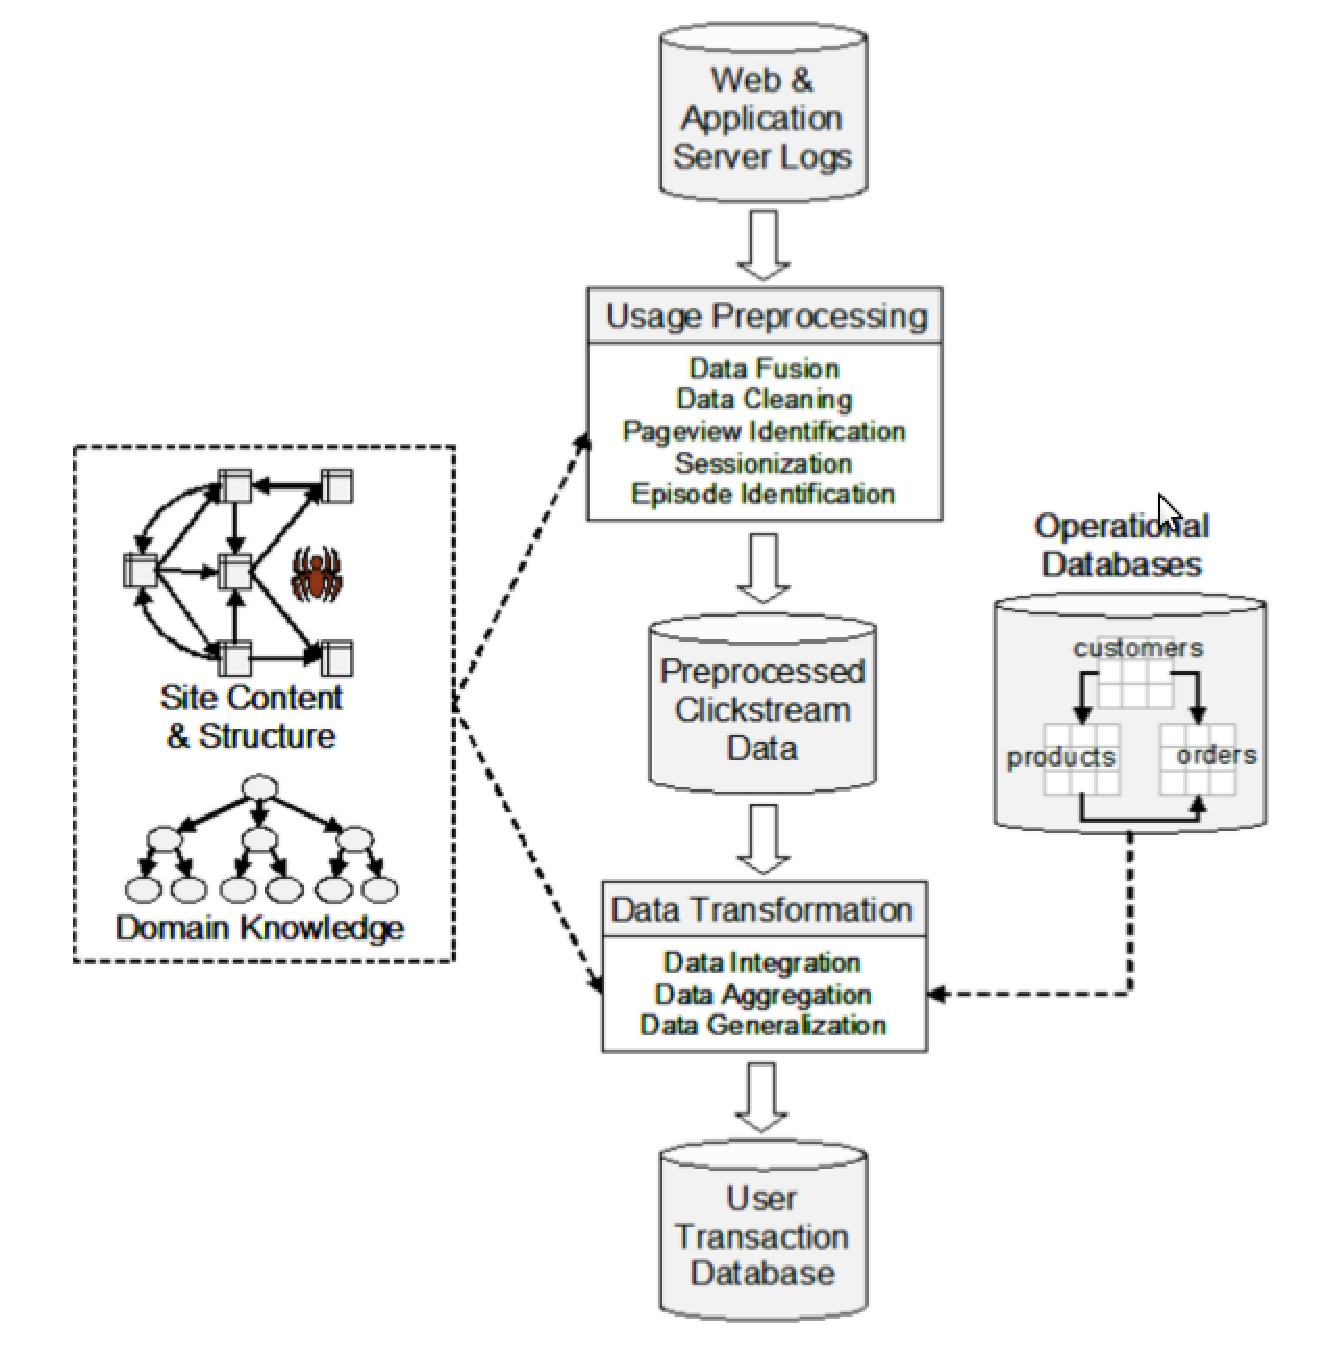
\includegraphics[scale=0.5]{step_1}
\caption{Estrutura do pré-processamento da mineração de uso}
\label{Rotulo}
\end{figure}


	Na segunda etapa, ou seja, descoberta do padrão, são usadas as estatísticas e base de dados, além da realização de operações de máquinas de aprendizagem para obter os padrões que estão escondidos, ocultos, que refletem no comportamento padrão dos usuários.

	Na última etapa, ou seja, análise de padrão, as estatísticas e os padrões encontrados na etapa anterior serão processados e filtrados para gerar um modelo de usuários agregados que poderão ser utilizados como entrada de dados para ferramentas de visualização e análise de Web, geração de relatórios ou mecanismos de recomendação.


\begin{figure}[!htb]
\centering
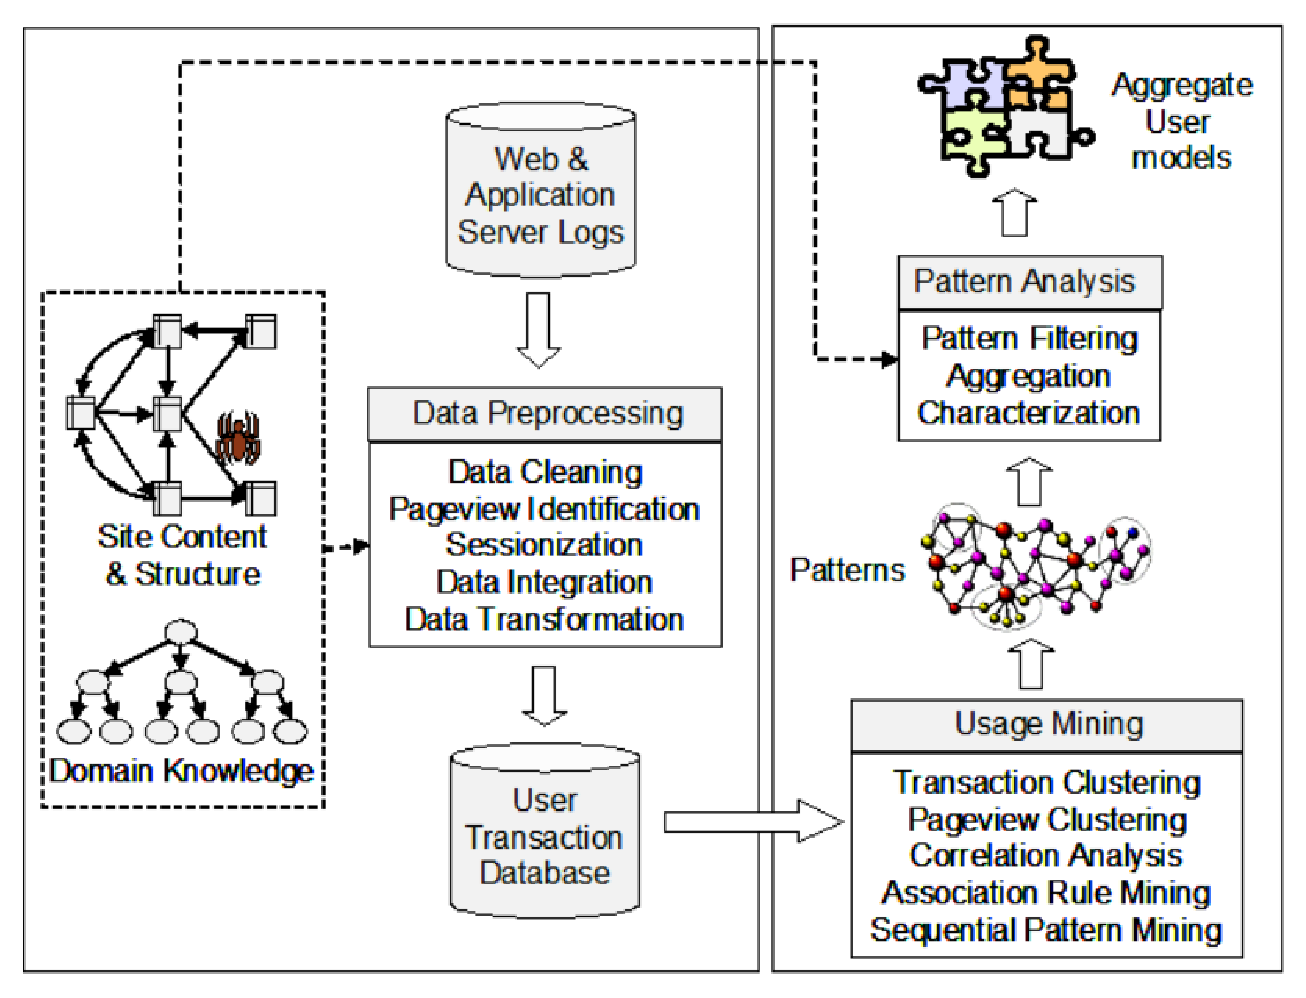
\includegraphics[scale=0.5]{mono_big}
\caption{Estrutura do processo geral de mineração de uso}
\label{Rotulo}
\end{figure}

